\documentclass{beamer}

\mode<presentation> {

% The Beamer class comes with a number of default slide themes
% which change the colors and layouts of slides. Below this is a list
% of all the themes, uncomment each in turn to see what they look like.

\usetheme{default}
%\usetheme{AnnArbor}
%\usetheme{Antibes}
%\usetheme{Bergen}
%\usetheme{Berkeley}
%\usetheme{Berlin}
%\usetheme{Boadilla}
%\usetheme{CambridgeUS}
%\usetheme{Copenhagen}
%\usetheme{Darmstadt}
%\usetheme{Dresden}
%\usetheme{Frankfurt}
%\usetheme{Goettingen}
%\usetheme{Hannover}
%\usetheme{Ilmenau}
%\usetheme{JuanLesPins}
%\usetheme{Luebeck}
%\usetheme[width=4in]{Madrid}
%\usetheme{Malmoe}
%\usetheme{Marburg}
%\usetheme{Montpellier}
%\usetheme{PaloAlto}
%\usetheme{Pittsburgh}
%\usetheme{Rochester}
%\usetheme{Singapore}
%\usetheme{Szeged}
%\usetheme{Warsaw}

% As well as themes, the Beamer class has a number of color themes
% for any slide theme. Uncomment each of these in turn to see how it
% changes the colors of your current slide theme.

%\usecolortheme{albatross}
%\usecolortheme{beaver}
%\usecolortheme{beetle}
%\usecolortheme{crane}
%\usecolortheme{dolphin}
%\usecolortheme{dove}
%\usecolortheme{fly}
%\usecolortheme{lily}
%\usecolortheme{orchid}
%\usecolortheme{rose}
%\usecolortheme{seagull}
%\usecolortheme{seahorse}
%\usecolortheme{whale}
%\usecolortheme{wolverine}

%\setbeamertemplate{footline} % To remove the footer line in all slides uncomment this line
\setbeamertemplate{footline}[page number] % To replace the footer line in all slides with a simple slide count uncomment this line

\setbeamertemplate{navigation symbols}{} % To remove the navigation symbols from the bottom of all slides uncomment this line
}
\renewcommand{\indent}{\hspace*{2em}}
\usepackage{graphicx} % Allows including images
\usepackage{booktabs} % Allows the use of \toprule, \midrule and \bottomrule in tables
%\usepackage {tikz}
\usepackage{tkz-graph}
\GraphInit[vstyle = Shade]
\tikzset{
  LabelStyle/.style = { rectangle, rounded corners, draw,
                        minimum width = 2em, fill = yellow!50,
                        text = red, font = \bfseries },
  VertexStyle/.append style = { inner sep=5pt,
                                font = \normalsize\bfseries},
  EdgeStyle/.append style = {->, bend left} }
\usetikzlibrary {positioning}
%\usepackage {xcolor}
\definecolor {processblue}{cmyk}{0.96,0,0,0}
%----------------------------------------------------------------------------------------
%	TITLE PAGE
%----------------------------------------------------------------------------------------

\title[Short title]{MTH9899 Final Project Presentation} % The short title appears at the bottom of every slide, the full title is only on the title page

\author{Yigao (Hugo) Liu, Haocheng (Frank) Gu,\\
        Chenyu (Phillip) Zhao, Zichao (David) Wang} % Your name
\institute[UC Riverside] % Your institution as it will appear on the bottom of every slide, may be shorthand to save space
{
Baruch College, CUNY \\ % Your institution for the title page
\medskip
}
\date{May 22, 2019} % Date, can be changed to a custom date

\begin{document}

\begin{frame}
\titlepage % Print the title page as the first slide
\end{frame}

\begin{frame}
\frametitle{Overview} % Table of contents slide, comment this block out to remove it
\tableofcontents % Throughout your presentation, if you choose to use \section{} and \subsection{} commands, these will automatically be printed on this slide as an overview of your presentation
\end{frame}

%----------------------------------------------------------------------------------------
%	PRESENTATION SLIDES
%----------------------------------------------------------------------------------------

%------------------------------------------------

\section{Trim Data}
\subsection{Correlation Heatmap and Histogram}
\begin{frame}{Correlation Heatmap}
\begin{figure}[ht]
\centering
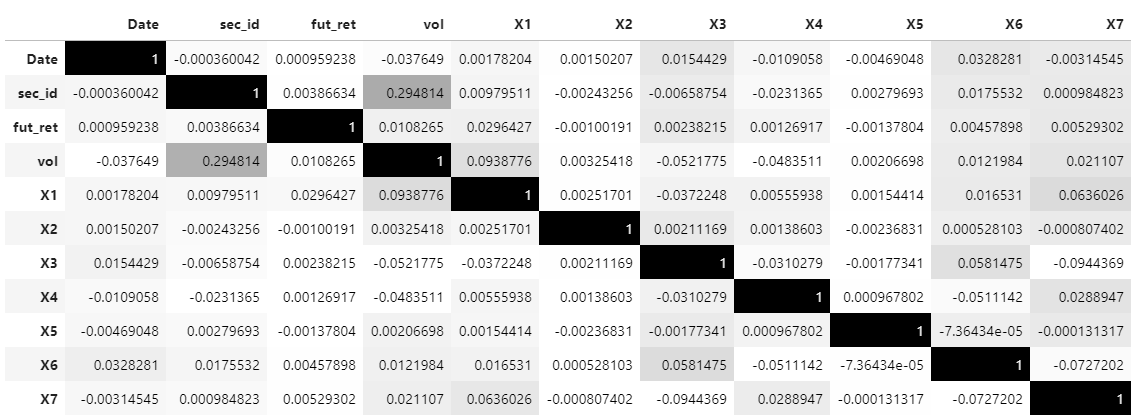
\includegraphics[scale=0.55]{corr_heatmap.PNG}
\caption{pairwise correlation heatmap}
\label{fig:label}
\end{figure}

\begin{itemize}
    \item "sec\_id" has a strong positive correlation with volatility.
\end{itemize}
\end{frame}

\begin{frame}{Population Histogram}
\begin{figure}[ht]
\centering
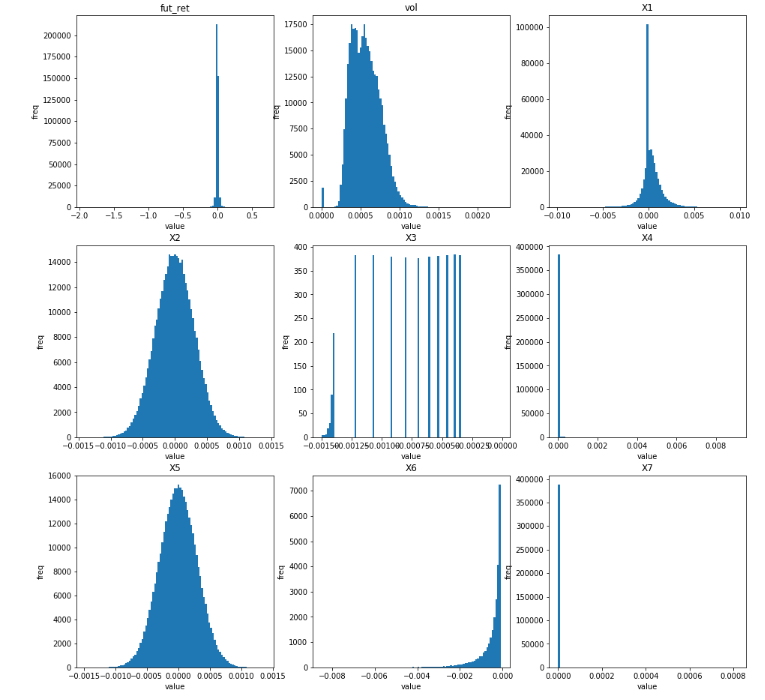
\includegraphics[scale=0.45]{pop_hist.PNG}
\caption{population histogram for each feature}
\label{fig:label}
\end{figure}

\begin{itemize}
    \item "X2" and "X5" are very likely to be pure white noise.
    \item "X1" seems to contain some information.
\end{itemize}
\end{frame}

\subsection{Features Dominated by Random Noise}
\begin{frame}{Moment Plot}
One way to further investigate whether a feature "X*" is noise is that for each ticker, we plot the 1st, 2nd and 3rd moment of "X*" across the time, and see if the value varies across each ticker.

\begin{itemize}
    \item If it does not vary, "X*" is probably noise.
    \item Otherwise "X*" may contain some information.
\end{itemize}
\end{frame}

\begin{frame}{Moment Plot}
\begin{figure}[ht]
\centering
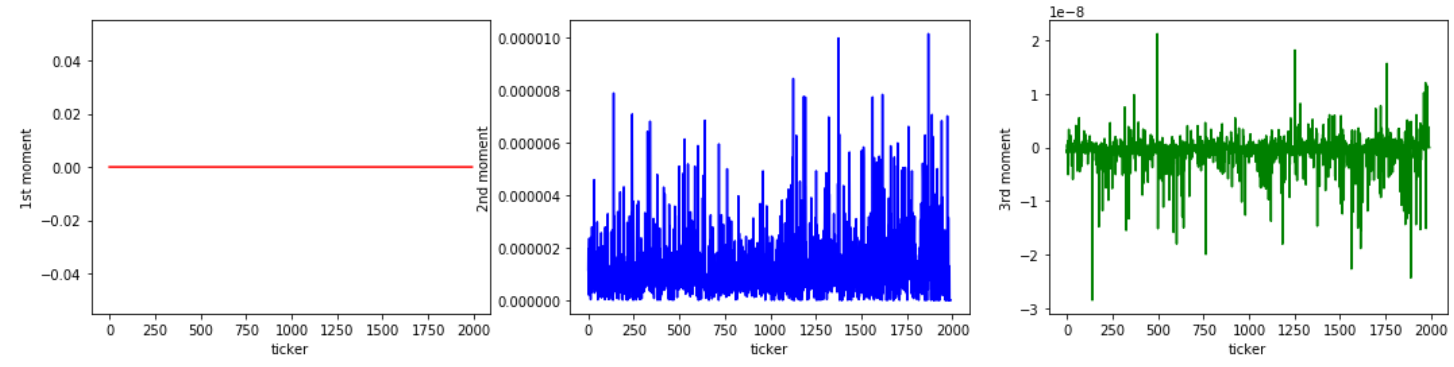
\includegraphics[scale=0.22]{moments_x1.PNG}
\caption{1st, 2nd and 3rd moments of "X1" across different tickers}
\label{fig:label}
\end{figure}

\begin{figure}[ht]
\centering
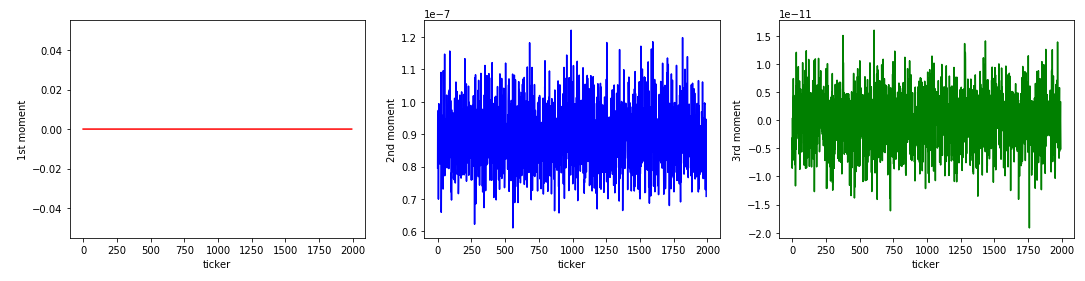
\includegraphics[scale=0.3]{moments_x2.PNG}
\caption{1st, 2nd and 3rd moments of "X2" across different tickers}
\label{fig:label}
\end{figure}

\begin{figure}[ht]
\centering
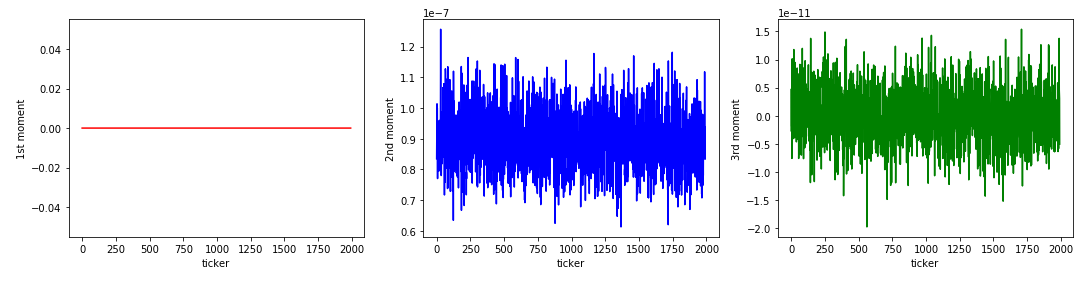
\includegraphics[scale=0.3]{moments_x5.PNG}
\caption{1st, 2nd and 3rd moments of "X5" across different tickers}
\label{fig:label}
\end{figure}
\end{frame}

\subsection{Deal with Missing Values}
\begin{frame}{Two Possibilities}
There are two most common possibilities for missing values in a time series:
\begin{itemize}
    \item[1.] A few np.nans lie among valid data in a time series.
    \item[2.] A big chunk of np.nans at the beginning (or in the middle) of our time period.
\end{itemize}

\noindent We can probably use some kind of moving average to fill the np.nans in case 1; but we have to treat case 2 more seriously.\\
\end{frame}

%\begin{frame}{np.nans in Features other than "vol".}
%Due to our discussion above, in different feature dataframes (such as "fut\_ret" and "X7"), all np.nans are in the same place. So if we fill the missing values using some moving average (such as exponential moving average), we will get $\frac{5861}{392539}\approx1.5\%$ of our data points among which all the features are just filled in artificially.\\
%\indent Thus we have to drop them in the end and leave the time stamps of different stocks somewhat not identical.
%\end{frame}

\begin{frame}{np.nans in "vol"}
\begin{itemize}
\item One way to fill np.nan is to use exponential moving average.
\item We calculate the moving average using historical data in order to avoid lookahead bias.
\item But there is one parameter we have to decide: the center of mass (or effective lag) of our moving average.
\item Therefore, we have to do some kind of parameter tuning.
\end{itemize}
\end{frame}

\begin{frame}{Tune with "sec\_id"}
\begin{figure}[ht]
\centering
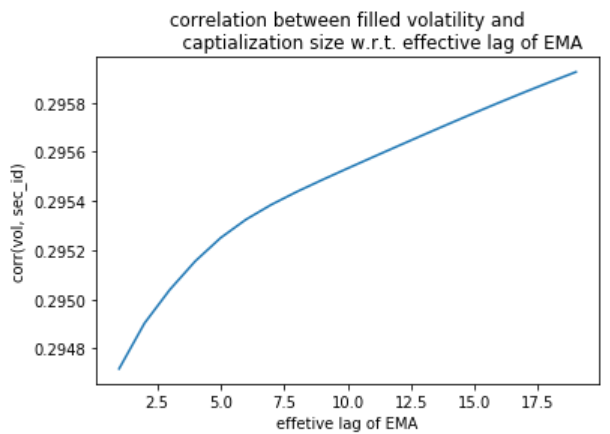
\includegraphics[scale=0.7]{corr_vol_sec_id.PNG}
\caption{correlation with EMA-filled vol w.r.t. sec\_id}
\label{fig:label}
\end{figure}
\begin{itemize}
\item We are disappointed to see that the correlation keeps going up, and a EMA with  $lag>15$ actually does not make sense.
\end{itemize}
\end{frame}

\begin{frame}{Tune with "X1"}
\begin{figure}[ht]
\centering
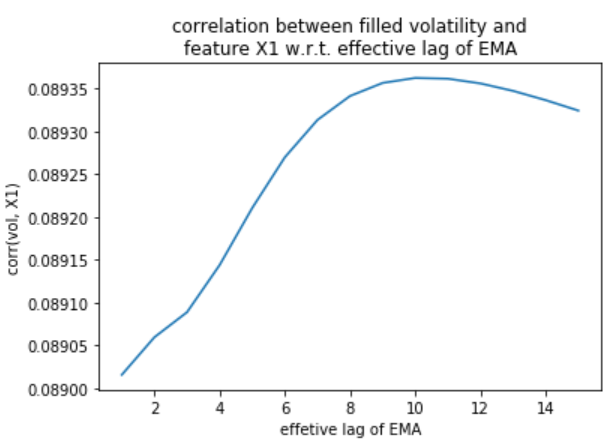
\includegraphics[scale=0.7]{corr_vol_x1.PNG}
\caption{correlation with EMA-filled vol w.r.t. sec\_id}
\label{fig:label}
\end{figure}
\begin{itemize}
\item{Based on this plot, we will choose $lag=10$.}
\end{itemize}
\end{frame}

\begin{frame}{Remaining np.nans in "vol"}
\begin{itemize}
    \item After filling in with exponential moving averages, we can find that there are still 20,887 np.nans in "vol".
\end{itemize}

\begin{figure}[ht]
\centering
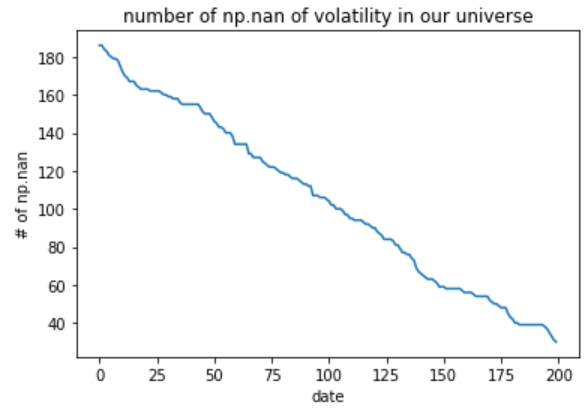
\includegraphics[scale=0.6]{num_of_nan.PNG}
\caption{number of np.nan of volatility w.r.t. date}
\label{fig:label}
\end{figure}

\begin{itemize}
    \item The most reasonable way tends to be the most naive one: just leave all np.nans unfilled.
\end{itemize}
\end{frame}

\subsection{Normalization}
\begin{frame}{Normalization}
 We set our features into four sets and treat them differently:
\begin{itemize}
    \item[1.] sec\_id, Date: we will divide each value by the sample maximum.
    \item[2.] X2, X5: we will not normalize them because we will drop them in the end anyway.
    \item[3.] vol: we will first add a minor positive number ($10^{-4}$) in order to avoid numerical error, and then take log and compute z-score. New feature will be named "log\_vol".
    \item[4.] X1, X3, X4, X6, X7: we will compute z-score of them directly. New features will be named "X*\_norm".
\end{itemize}
\end{frame}


%%%%%%%%%%%%%%%%%%%%%%%%%%%%%%%%%%%%%%%%%%%%%%%%%%%%%%%%%%%%%%%%%
%%%%%%%%%%%%%%%%%%%%%%%%%%%%%%%%%%%%%%%%%%%%%%%%%%%%%%%%%%%%%%%%%
\section{Regression Analysis}
\subsection{Regression}
\begin{frame}{Different Regressions}
\begin{itemize}
    \item Models: OLS, +/- 4MADs, OLS on the strongest signal, OLS by large and small SECID, LASSO, Ridge.
    \item Experiment: LightGBM.
\end{itemize}

\begin{figure}[ht]
\centering
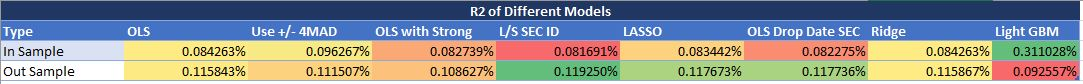
\includegraphics[scale=0.4]{Regression_Performance_V2.JPG}
\caption{$R^{2}$ of Different Models}
\label{fig:label}
\end{figure}

\end{frame}



\begin{frame}{Prediction vs. Actual}
\begin{figure}[ht]
    \centering
    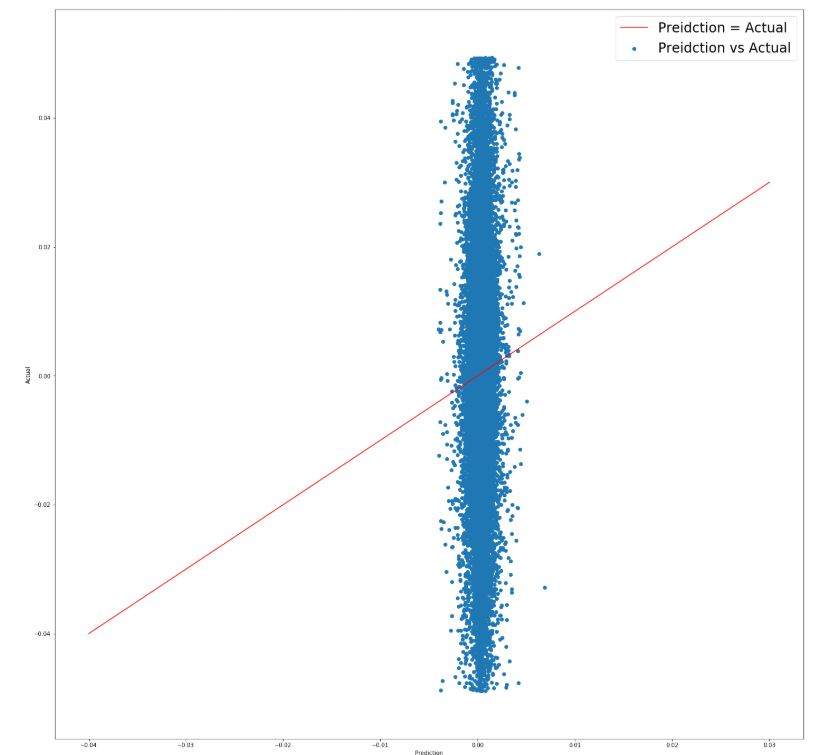
\includegraphics[scale=0.3]{Reg_Pred_vs_Act.JPG}
    \caption{Prediction vs Actual}
    \label{fig:label}
\end{figure}

\end{frame}


\begin{frame}{LASSO}
\begin{itemize}
    \item Date and SECID reach 0 first.
    \item X1 last till the end.
\end{itemize}

\begin{figure}[ht]
    \centering
    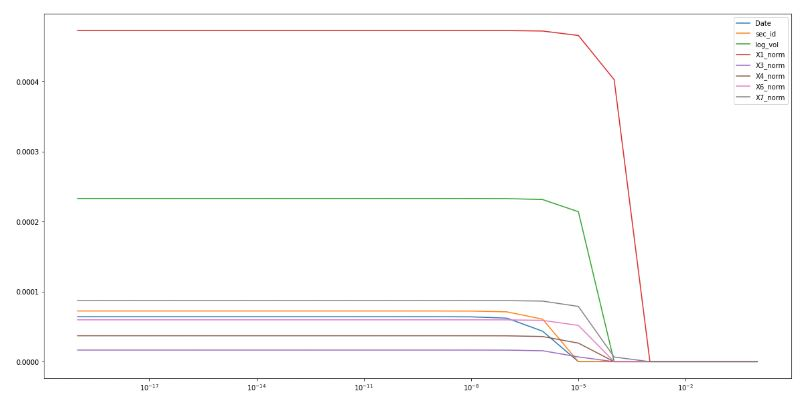
\includegraphics[scale=0.5]{LASSO.JPG}
    \caption{Coefficients of Variables as Penalty Increases}
    \label{fig:label}
\end{figure}

\end{frame}

%%%%%%%%%%%%%%%%%%%%%%%%%%%%%%%%%%%%%%%%%%%%%%%%%%%%%%%%%%%%%%%%%

\section{Tree Models}
\begin{frame}{Tree Models}
\begin{itemize}
    \item Default tree
    \item Default random forest
    \item Self-defined tree
    \item Self-defined forest
\end{itemize}
\end{frame}

\subsection{Default Tree \& Forest}
\begin{frame}{Default Tree}
\begin{itemize}
    \item Randomly split
    \item Cross validation on depth
    \item Other parameters
\end{itemize}

\begin{figure}[ht]
        \centering
        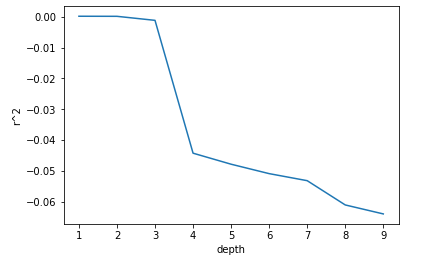
\includegraphics[width=0.7\linewidth,height=0.4\linewidth]{depth_default_tree.png}
        \caption{depth of default tree}
        \label{fig:label}
    \end{figure}
\end{frame}

\begin{frame}{Default Forest}
\begin{itemize}
    \item Use 3 as the best depth
    \item Cross validation on the numbers of trees
    \item Other parameters
\end{itemize}

\begin{figure}[htbp]

\subfigure{
\begin{minipage}[t]{0.4\linewidth} 
\centering 
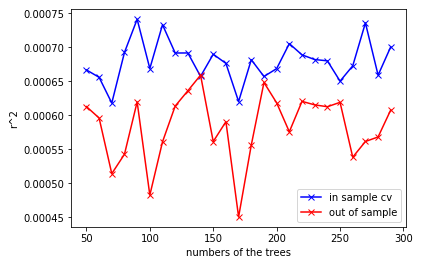
\includegraphics[width=1.8in]{cv_and_r^2_for_forest.png} 
\caption{cv and $r^2$}
\end{minipage}}
\subfigure{
\begin{minipage}[t]{0.4\linewidth} 
\centering 
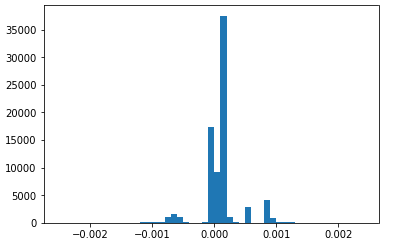
\includegraphics[width=1.8in]{hist_default_tree.png} 
\caption{hist of output}
\end{minipage}}

\end{figure}
We can see that the performance is not very good, and the predictions are just the mean.
\end{frame}

\subsection{Self-defined Tree \& Forest}
\begin{frame}{Self-defined Tree}
\begin{itemize}
    \item For each feature, distinguish zero from non-zero values first
    \item Cross validation on the depth
    \item Other parameters
\end{itemize}

\begin{figure}[ht]
        \centering
        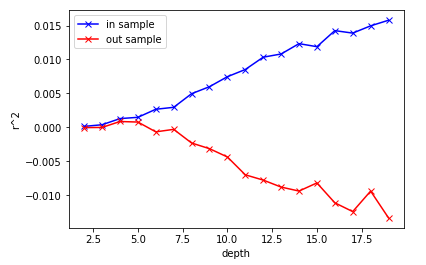
\includegraphics[width=0.7\linewidth,height=0.4\linewidth]{depth_our_tree.png}
        \caption{depth of self-defined tree}
        \label{fig:label}
    \end{figure}
\end{frame}


\begin{frame}{Self-defined Forest}
\begin{itemize}
    \item Use 7 as the best depth
    \item Cross validation on the numbers of trees
    \item Other parameters
\end{itemize}

\begin{figure}[htbp]

\subfigure{
\begin{minipage}[t]{0.4\linewidth} 
\centering 
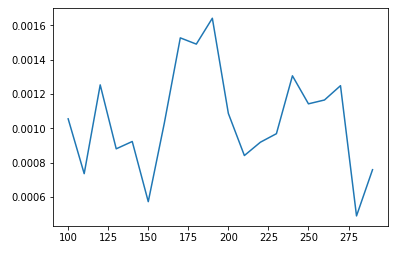
\includegraphics[width=1.8in]{cv_our_tree.png} 
\caption{cv of our tree}
\end{minipage}}
\subfigure{
\begin{minipage}[t]{0.4\linewidth} 
\centering 
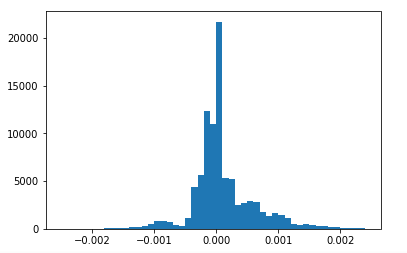
\includegraphics[width=1.8in]{hist_our_tree.png} 
\caption{hist of output}
\end{minipage}}

\end{figure}
We can see that the performance is better than before. Although there are still many predictions which give the mean value, we can see a fat tail in this picture. The average out-of-sample $r^2$ is 13 bps. 
\end{frame}

\begin{frame}{Adding More Randomness}
\begin{itemize}
    \item Randomly select 3 features to split on each point.
\end{itemize}

\begin{figure}[ht]
        \centering
        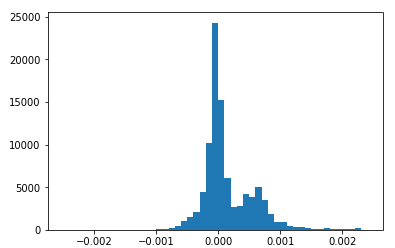
\includegraphics[width=0.7\linewidth,height=0.4\linewidth]{hist_of_random.png}
        \caption{hist of output}
        \label{fig:label}
    \end{figure}

We can see that the performance is still better than default.The shape of histogram is almost the same as before, but the average out-of-sample $r^2$ is 10 bps. 
\end{frame}
%%%%%%%%%%%%%%%%%%%%%%%%%%%%%%%%%%%%%%%%%%%%%%%%%%%%%%%%%%%%%%%%%
\section{Neural Network}
\begin{frame}{Neutral Network and its results}
    I applied different variations of Neural Networks to different variations of data set, turned out no good result benefited from deep net structure.
    \begin{itemize}
        \item NN can not capture fat-tail of return distribution, under scale of original data.
        \item There is no good metrics, NN behaves poor in both train and test set.
        \item Best test R-square is between 7 to 12 bps, when framework is very simple
        \item When build it deep, NN tends to predict the mean value
    \end{itemize}
\end{frame}

\begin{frame}{Histogram}
    \begin{figure}[ht]
        \centering
        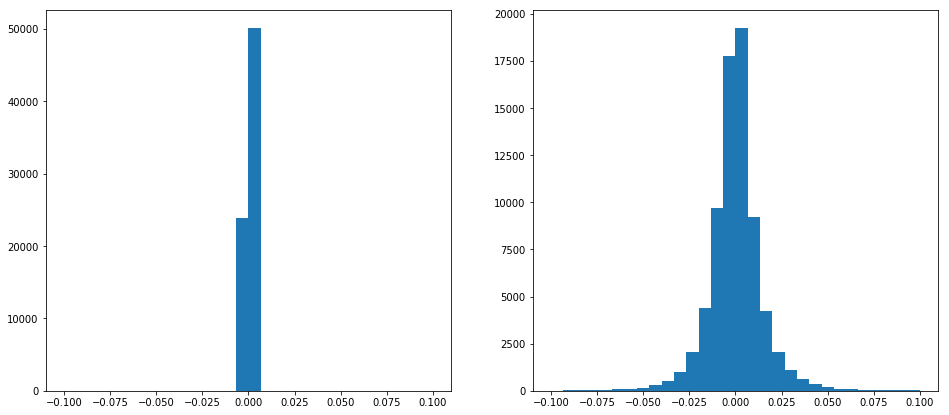
\includegraphics[width=0.7\linewidth,height=0.2\linewidth]{NN_1.png}
        \caption{Best Prediction / True results}
        \label{fig:label}
    \end{figure}
    
     \begin{figure}[ht]
        \centering
        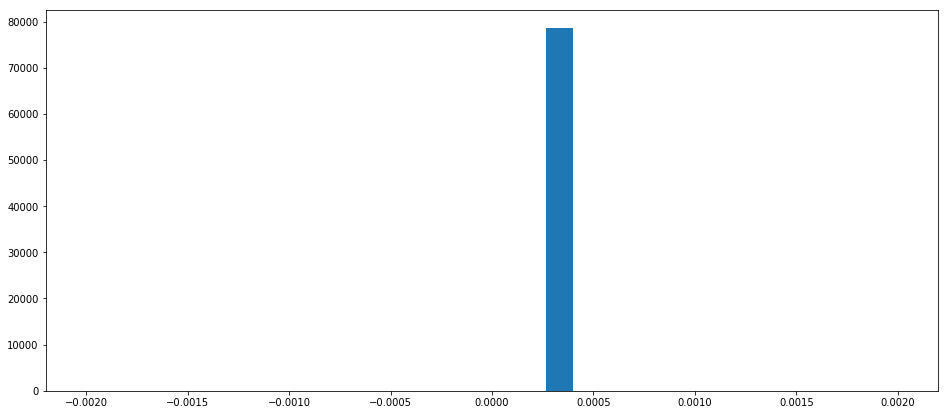
\includegraphics[width=0.7\linewidth,height=0.2\linewidth]{NN_2.png}
        \caption{Deep NN's Prediction}
        \label{fig:label}
    \end{figure}
\end{frame}

\begin{frame}{What I tried}
    \begin{itemize}
        \item Structure: linear fully connected NN, up to 5 layers, 128 neurons each
        \item Optimizer: Adam
        \item Different learning rates
        \item Activation function: ReLU, leaky ReLU, Tanh
        \item Drop layer: randomly inactivate 0.5 portion of neurons in each epoch
        \item Batch normalization layer: normalize output after each layer
        \item L2 regularization: on weights of neurons
    \end{itemize}
\end{frame}

\begin{frame}{Best network}
\begin{itemize}
    \item single layer, 4 neurons
    \item no drop layer
    \item L2 regularization: 0.1
    \item leaky ReLU
    \item do batch normalization
    \item use sec\_id, X1\_norm, X3
    \item to predict fut\_ret/vol
\end{itemize}
    Can basically predict rise or drop. R-square between 7 and 12 bps in both test and train sets.
  
\end{frame}

%%%%%%%%%%%%%%%%%%%%%%%%%%%%%%%%%%%%%%%%%%%%%%%%%%%%%%%%%%%%%%%%%
%%%%%%%%%%%%%%%%%%%%%%%%%%%%%%%%%%%%%%%%%%%%%%%%%%%%%%%%%%%%%%%%%
\section{Aggregation}
\begin{frame}{Aggregation}
\begin{itemize}

\item For aggregating, firstly we trained all existing models under first 150 days. Then these models gave predictions for latter 50 days.

\item Now we want to use these predictions from existing models as input for an upper-level model. This upper-level model will combine all results from existing models. 

\item We split these 50 days into 3:1 portion as training and test set for this upper-level model.

\item Note that the training set for this upper-level is the test set from lower-level. From this point, training or test is in sense of upper-level model.

\end{itemize}
\end{frame}
\begin{frame}{How to deal with NaN in vol}
    We used two different ways to deal with NaN in vol.
    \begin{itemize}
        \item First way: We fill all NaN with 0.
        \item Second way: We treat data with NaN vol as another group of data. We assume it has different property from other data. Under this consumption we build our two-level model only on non-NaN-vol data, and build another simple model for NaN-vol data. 
        \item For the latter simple model we use linear regression on all other features, instead of just fill 0 in return prediction. Because we don't want to assume any extra things. Linear model is most explainable, so we choose it.
        \item Actually we model two kinds of data separately and combine them together
    \end{itemize}
    These two methods has close performance up to lower-level. But when we do aggregation, we found the second one has much better r-square. Though the second way maybe have data-driven suspicion, latter we will focus on this method.
\end{frame}

\begin{frame}{Existing model}
    \begin{figure}[ht]
        \centering
        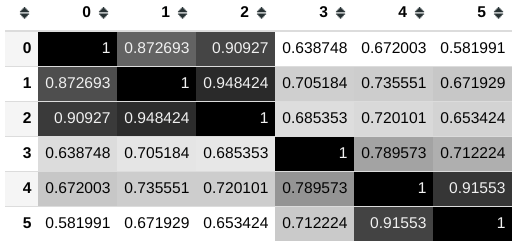
\includegraphics[width=0.7\linewidth,height=0.4\linewidth]{agg_1.png}
        \caption{Correlations between features in train set}
        \label{fig:label}
    \end{figure}
    
    The existing models from lower-level are Neural Network, OLS1, OLS2,  Ridge, Light GBM, Random Forest1, Random Forest2  
\end{frame}

\begin{frame}{Agg method}
\begin{itemize}
    \item Neutral Network: Even after the simplest net, the prediction is mean of data.
    \item OLS: Bad approach, as there is high correlation between features
    \item Lasso: very small penalty(1e-7) leads to choose only one feature. We let it choose two features.
    \item Ridge: Best results cannot beat Lasso.
    \item Random Forest: Very amazing!
    \item Light GBM: Not amazing.
\end{itemize}
As usual, all models' hyper parameter tuned with cross validation.
\end{frame}

\begin{frame}{Results}
    \begin{figure}[ht]
        \centering
        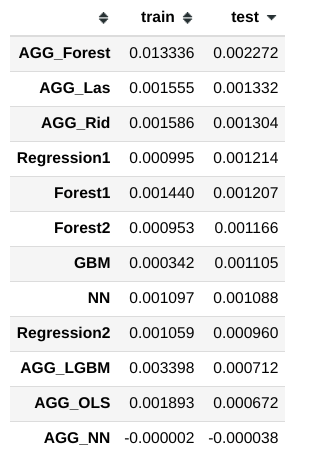
\includegraphics[width=0.7\linewidth,height=0.7\linewidth]{agg_2.png}
        \caption{Results(in order of test R2)}
        \label{fig:label}
    \end{figure}
\end{frame}

\begin{frame}{Conclusion}
    So aggregating did give us better result. So we choose Random Forest aggregation with 6 other models as our final choice.

    feature importance:
    \begin{itemize}
        \item NN: 0.26931832
        \item Regression 1: 0.1825856
        \item Random Forest 1: 0.17319282
        \item Random Forest 2:0.14946527
        \item Regression 2: 0.13878568
        \item Light GBM: 0.08665231
    \end{itemize}

Under this method we can achieve 23 bps while the first fill-NA-with-zero way can achieve 13 bps.
\end{frame}

\begin{frame}{Results}
    \begin{figure}[ht]
        \centering
        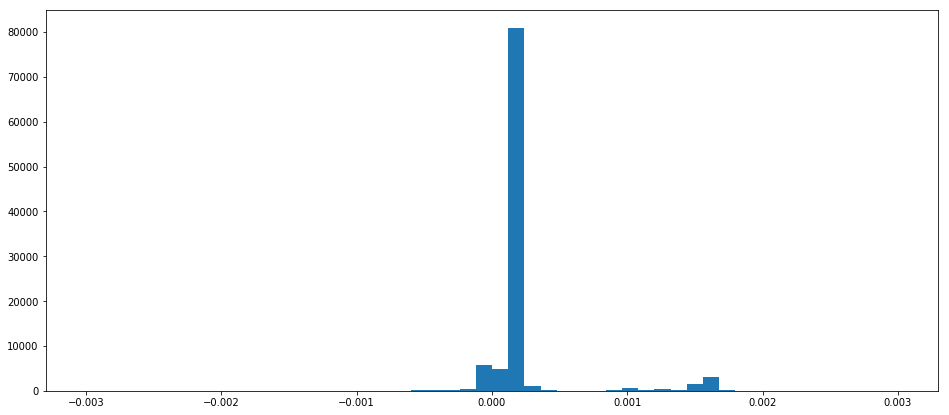
\includegraphics[width=0.7\linewidth,height=0.7\linewidth]{agg_5.png}
        \caption{oos prediction histogram}
        \label{fig:label}
    \end{figure}
\end{frame}


%%%%%%%%%%%%%%%%%%%%%%%%%%%%%%%%%%%%%%%%%%%%%%%%%%%%%%%%%%%%%%%%%%%%%%%5
\begin{frame}
\Huge{\centerline{Thanks for Listening}}
\end{frame}

\end{document}
%----------------------------------------------------------------------------------------
